\documentclass[slidestop,compress,xcolor=table,mathserif,hyperref={bookmarks=false}]{beamer}
\usetheme{TACC}

\usepackage{tikz}
\usetikzlibrary{automata,shapes,arrows}
\usepackage{lmodern}
\usepackage[overlay]{textpos}
\usepackage[applemac]{inputenc}
\usepackage{pgfpages}
\usepackage{multirow}

\newenvironment<>{varblock}[2][.9\textwidth]{
  \setlength{\textwidth}{#1}
  \begin{actionenv}#3
    \def\insertblocktitle{#2}
    \par
    \usebeamertemplate{block begin}}
  {\par
    \usebeamertemplate{block end}
  \end{actionenv}}

\author{\textbf{\Large Jim Browne, Ashay Rane and Leo Fialho}}
\begin{document}

\AtBeginSection[]{
	\frame<beamer>{
		\frametitle{Agenda}
		\begin{columns}[c]
			\begin{column}{0.6\textwidth}
				\tableofcontents[currentsection,subsectionstyle=shadow/hide/hide]
			\end{column}
			\begin{column}{0.5\textwidth}
				\pgfuseimage{configuration}
			\end{column}
		\end{columns}
	}
}

%------------------------------------------------------------
\pgfdeclareimage[interpolate=true,width=5cm]{logo_TACC}{figures/tacc}
\pgfdeclareimage[interpolate=true,width=5cm]{logo_UT}{figures/ut}
\pgfdeclareimage[interpolate=true,width=1.5cm]{logo_TACC_small}{figures/tacc}
\pgfdeclareimage[interpolate=true,width=1cm]{logo_UT_small}{figures/ut}
\pgfdeclareimage[interpolate=true,width=6cm]{configuration}{figures/configuration}

%------------------------------------------------------------
\title{\textbf{\Huge PerfExpert}}
\date{\textbf{\huge Petascale Tools Workshop\\Madison WI, 2013} \\ \ \\ \ \\ \pgfuseimage{logo_TACC} \ \ \pgfuseimage{logo_UT}}
\logo{\pgfuseimage{logo_TACC_small} \ \ \ \pgfuseimage{logo_UT_small}}
\frame[plain]{\titlepage}

%------------------------------------------------------------
\section{Introduction}

\subsection{Overview}
\frame{\frametitle{Overview: why PerfExpert?} %\pause
	\begin{block}{Problem: HPC systems operate far below peak} %\pause
		\begin{itemize}
			\item Chip/node architectural complexity is growing rapidly \\[2mm] %\pause
			\item Performance optimization for these chips requires deep knowledge of architectures, code patterns, compilers, etc. \\[2mm]
		\end{itemize}
	\end{block}
	\begin{exampleblock}{Performance optimization tools} %\pause
		\begin{itemize}
			\item Powerful in the hands of experts \\[2mm] %\pause
			\item Require detailed performance and system expertise \\[2mm] %\pause
			\item HPC application developers are domain experts, not computer gurus \\[2mm] %\pause
		\end{itemize}
	\end{exampleblock}
	\begin{alertblock}{Many HPC programmers/users do not use your tools}
		\centering (seriously)
	\end{alertblock}
}

\frame{\frametitle{Goal for PerfExpert: democratize optimization!} %\pause
	\begin{block}{Subgoals:} %\pause
		\begin{itemize}
			\item Make use of the tool as simple as possible \\[2mm] %\pause
			\item Start with only chip/node level optimization \\[2mm] %\pause
			\item Make it adaptable across multiple architectures \\[2mm] %\pause
%			\item Design for extension to communication and I/O performance \\[0mm] %\pause
		\end{itemize}
	\end{block}
	\begin{exampleblock}{How to accomplish?} %\pause
		\begin{itemize}
			\item Formulate the performance optimization task as a workflow of subtasks \\[2mm] %\pause
			\item Leverage the state-of-the-art: build on the best available tools for the subtasks to minimize the effort and cost of development \\[2mm] %\pause
			\item Automate the entire workflow \\[2mm] %\pause
		\end{itemize}
	\end{exampleblock}
}

\subsection{Introduction}
\frame{\frametitle{Introduction}
	\begin{block}{The four stages of automatic performance optimization:} %\pause
		\begin{itemize}
			\item Measurement and attribution (1) \\[2mm] %\pause
			\item Analysis, diagnosis and identification of bottlenecks (2) \\[2mm] %\pause
			\item Selection of effective optimizations (3) \\[2mm] %\pause
			\item Implementation of optimizations (4) \\[2mm] %\pause
		\end{itemize}
	\end{block}

	\begin{exampleblock}{Use of State-of-the-Art:} %\pause
		\begin{itemize}
			\item HPCToolkit/Intel VTune, \textbf{MACPO} based on ROSE (1) \\[2mm] %\pause
			\item \textbf{PerfExpert Team} (2 and 3) \\[2mm] %\pause
			\item \textbf{PerfExpert Team} based on ROSE, PIPS, Bison and Flex (4)\\[2mm] %\pause
		\end{itemize}
	\end{exampleblock}
}

\frame{\frametitle{Introduction}
	\begin{block}{Uniqueness of PerfExpert:} %\pause
		\begin{itemize}
			\item Nearly complete optimization first three stages of optimization for chip/node level \\[2mm] %\pause
			\item Framework for implementing optimizations is complete and several optimizations are completed \\[2mm] %\pause
			\item Integrates code segment focused and data structure based measurements (\textbf{MACPO})\\[1mm] %\pause
			--- Code segment local measurement \\[1mm] %\pause
			--- Data structure specific traces \\[1mm] %\pause
%			--- Order of magnitude lower overhead of measurement \\[1mm] %\pause
			--- More accurate (associative) cache models \\[1mm] %\pause
			--- Strides by data structure and code segment \\[1mm] %\pause
			--- Architecture ``independent'' metrics \\[1mm]
%			\item Workflow will apply to communication and I/O optimization as well \\[2mm] %\pause
		\end{itemize}
	\end{block}
}

%\frame{\frametitle{Introduction}
%	\begin{block}{Unique properties of MACPO (integrated into PerfExpert):} %\pause
%		\begin{itemize}
%			\item Multicore resolved traces \\[2mm] %\pause
%			\item Code segment local measurement \\[2mm] %\pause
%			\item Data structure specific traces \\[2mm] %\pause
%			\item Order of magnitude lower overhead of measurement \\[2mm] %\pause
%			\item More accurate (associative) cache models \\[2mm] %\pause
%			\item Strides by data structure and code segment \\[2mm] %\pause
%			\item Architecture ``independent'' metrics \\[2mm]
%		\end{itemize}
%	\end{block}
%}

\subsection{What can PerfExpert provide to you?}

\frame{\frametitle{What can PerfExpert provide to you?}
	\begin{block}{Performance report:} %\pause
		\begin{itemize}
			\item Identification of bottlenecks by relevance \\[2mm] %\pause
			\item Performance analysis based on performance metrics \\[2mm] %\pause
			\item Recommendations for optimization \\[2mm] %\pause
		\end{itemize}
	\end{block}

	\begin{exampleblock}{There are three possible outputs:} %\pause
		\begin{itemize}
			\item Performance report only \\[2mm] %\pause
			\item List of recommendations \\[2mm] %\pause
			\item Fully automated code transformation \\[2mm]
		\end{itemize}
	\end{exampleblock}
}

\frame{\frametitle{Performance Report}
	\begin{block}{}
\texttt{\tiny Loop in function compute() at mm.c:8 (99.8\% of the total runtime)\\
===============================================================================\\
ratio to total instrns \ \ \ \ \ \ \%  0.........25...........50.........75........100\\
\ \ \ - floating point \ \ \ \ \ : \ 100 ***********************************************\\
\ \ \ - data accesses \ \ \ \ \ \ : \ \ 25 ************\\
* GFLOPS (\% max) \ \ \ \ \ \ \ \ : \ \ 12 ******\\
\ \ \ - packed \ \ \ \ \ \ \ \ \ \ \ \ \ : \ \ \ 0 *\\
\ \ \ - scalar \ \ \ \ \ \ \ \ \ \ \ \ \ : \ \ 12 ******\\
-------------------------------------------------------------------------------\\
performance assessment \ \ \ \ \ LCPI good......okay......fair......poor......bad....\\
* overall \ \ \ \ \ \ \ \ \ \ \ \ \ \ \ : \ 3.0 >>>>>>>>>>>>>>>>>>>>>>>>>>>>>>>>>>>>>>>>>>>>>>+\\
upper bound estimates\\
* data accesses \ \ \ \ \ \ \ \ \ : \ 9.6 >>>>>>>>>>>>>>>>>>>>>>>>>>>>>>>>>>>>>>>>>>>>>>+\\
\ \ \ - L1d hits \ \ \ \ \ \ \ \ \ \ \ : \ 0.9 >>>>>>>>>>>>>>>>>\\
\ \ \ - L2d hits \ \ \ \ \ \ \ \ \ \ \ : \ 1.8 >>>>>>>>>>>>>>>>>>>>>>>>>>>>>>>>>>>>>\\
\ \ \ - L2d misses \ \ \ \ \ \ \ \ \ : \ 6.9 >>>>>>>>>>>>>>>>>>>>>>>>>>>>>>>>>>>>>>>>>>>>>>+\\
* instruction accesses \ \ : \ 0.1 >\\
\ \ \ - L1i hits \ \ \ \ \ \ \ \ \ \ \ : \ 0.0 >\\
\ \ \ - L2i hits \ \ \ \ \ \ \ \ \ \ \ : \ 0.0 >\\
\ \ \ - L2i misses \ \ \ \ \ \ \ \ \ : \ 0.1 >\\
* data TLB \ \ \ \ \ \ \ \ \ \ \ \ \ \ : \ \ 4.6 >>>>>>>>>>>>>>>>>>>>>>>>>>>>>>>>>>>>>>>>>>>>>>+\\
* instruction TLB \ \ \ \ \ \ \ : \ \ 0.0 >\\
* branch instructions \ \ \ : \ 0.1 >>\\
\ \ \ - correctly predicted : \ 0.1 >>\\
\ \ \ - mispredicted \ \ \ \ \ \ \ : \ 0.0 >\\
* floating-point instr \ \ : \ 5.1 >>>>>>>>>>>>>>>>>>>>>>>>>>>>>>>>>>>>>>>>>>>>>>+\\
\ \ \ - fast FP instr \ \ \ \ \ \ : \ 5.1 >>>>>>>>>>>>>>>>>>>>>>>>>>>>>>>>>>>>>>>>>>>>>>+\\
\ \ \ - slow FP instr \ \ \ \ \ \ : \ 0.0 >\\
}
   \end{block}
}

\frame{\frametitle{List of Recommendations}
	\begin{block}{}
\texttt{\small \#--------------------------------------------------\\
\# Recommendations for mm.c:8\\
\#--------------------------------------------------\\
\# This is a possible recommendation for this code segment\\
\#\\
Description: change the order of loops\\
Reason: this optimization may improve the memory access pattern and make it more cache and TLB friendly\\
Pattern Recognizers: c\_loop2 f\_loop2 \\
Code example:\\
loop i \{\\
\ \ loop j \{...\}\\
\}\\
 =====>
loop j \{\\
\ \ loop i \{...\}\\
\}\\
}
	\end{block}
}

\frame{\frametitle{Fully Automated Code Transformation}
	\begin{columns}[c]
		\begin{column}{0.5\textwidth}
			\begin{block}{Before:}
\texttt{\scriptsize void compute() \{\\
\ register int i, j, k;\\
\ \\
\ \\
\ \\
\ \\
\ \\
\ for (i = 0; i < 1000; i++)\\
\ \\
\ \\
\ \ for (j = 0; j < 1000; j++)\\
\ \\
\ \ \ for (k = 0; k < 1000; k++)\\
\ \ \ \ c[i][j] += (a[i][k] * b[k][j]);\\
\}\\
}
			\end{block}
		\end{column}
		\begin{column}{0.5\textwidth}
			\begin{block}{After:}
\texttt{\scriptsize void compute() \{\\
\ register int i, j, k;\\
\textcolor{red}{\ //PIPS generated variable}\\
\textcolor{red}{\ register int jp, kp;}\\
\textcolor{red}{\ /* PERFEXPERT: start work here */}\\
\textcolor{red}{\ /* PERFEXPERT: grandparent loop */}\\
\textcolor{red}{\ loop\_6:}\\
\textcolor{blue}{\ for (i = 0; i <= 999; i++)}\\
\textcolor{red}{\ \ /* PERFEXPERT: parent loop */}\\
\textcolor{red}{\ \ loop\_7:}\\
\textcolor{blue}{\ \ for(jp = 0; jp <= 999; jp += 1)}\\
\textcolor{red}{\ \ \ /* PERFEXPERT: bottleneck */}\\
\textcolor{blue}{\ \ \ for(kp = 0; kp <= 999; kp += 1)}\\
\textcolor{blue}{\ \ \ c[i][kp] += a[i][jp]*b[jp][kp];}\\
\}\\
}
			\end{block}
		\end{column}
	\end{columns}
}

%------------------------------------------------------------
\section{PerfExpert Modular Architecture}
\subsection{How PerfExpert does that?}

\frame{\frametitle{Current Version: The Big Picture}
	\begin{picture}(0,0)(0,0)
		\put(-28,-160){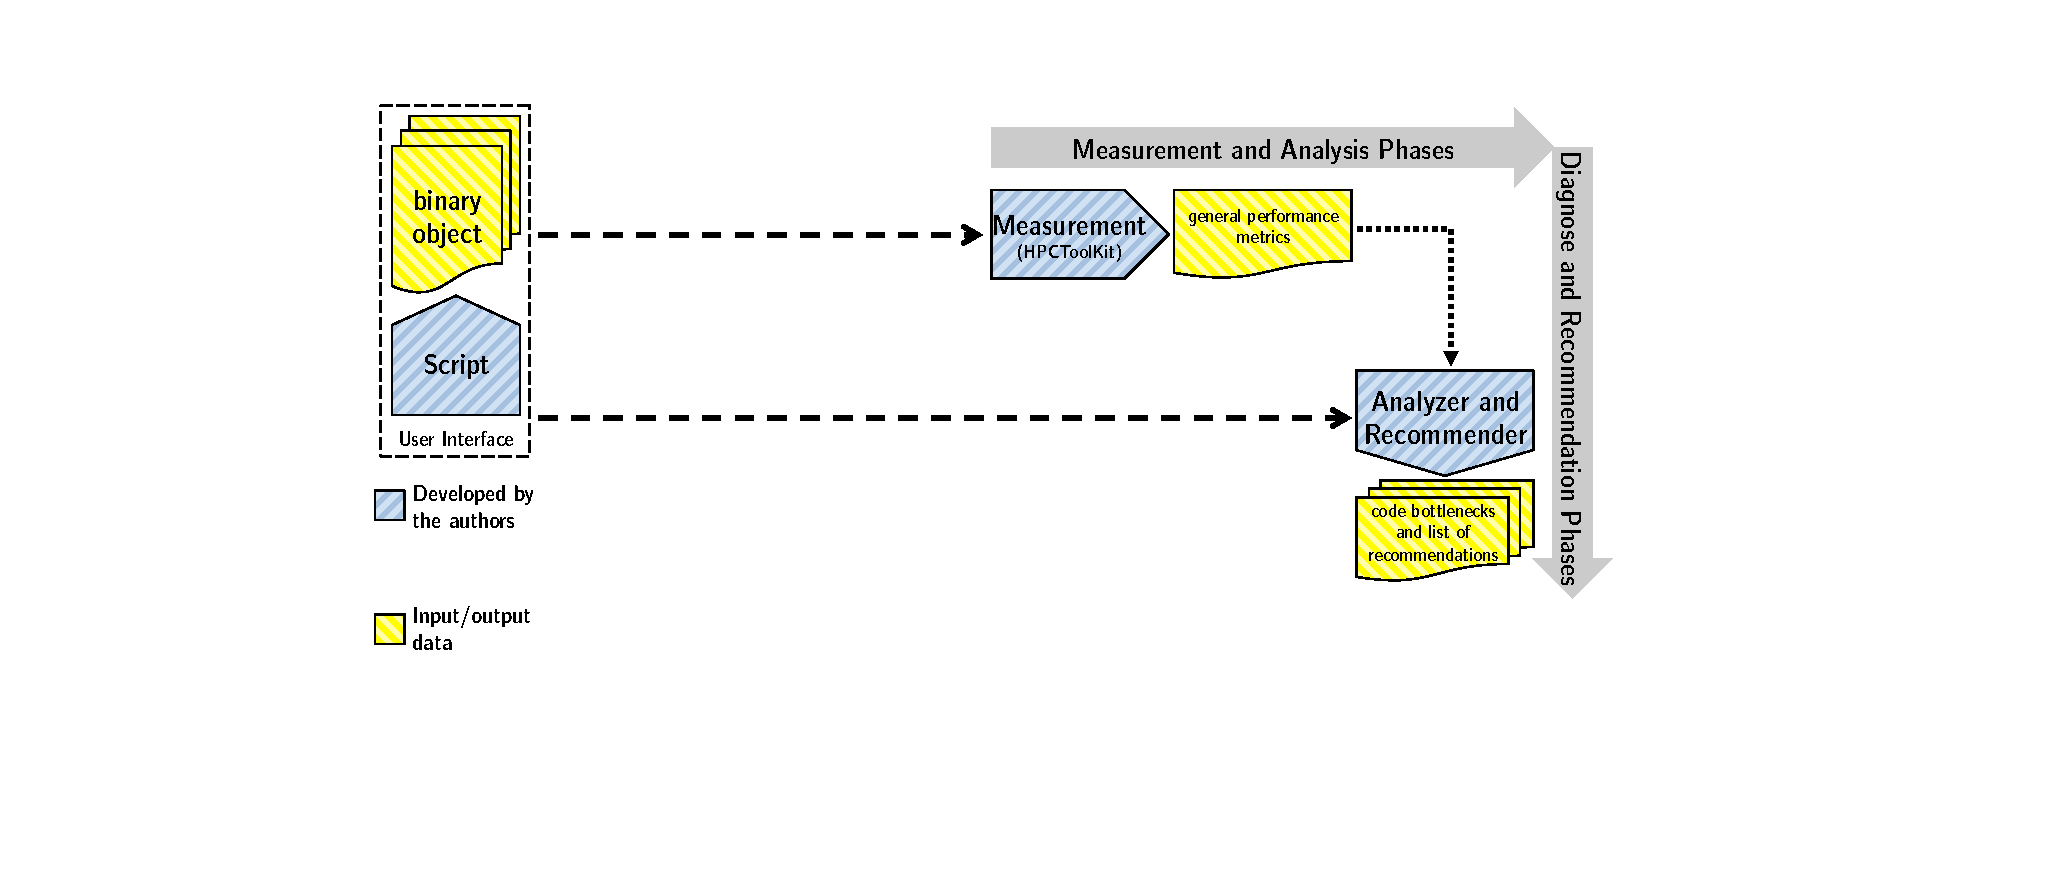
\includegraphics[width=12.8cm]{figures/pe_before}}
	\end{picture}
}

\frame{\frametitle{New Version: The Big Picture}
	\begin{picture}(0,0)(0,0)
		\put(-28,-160){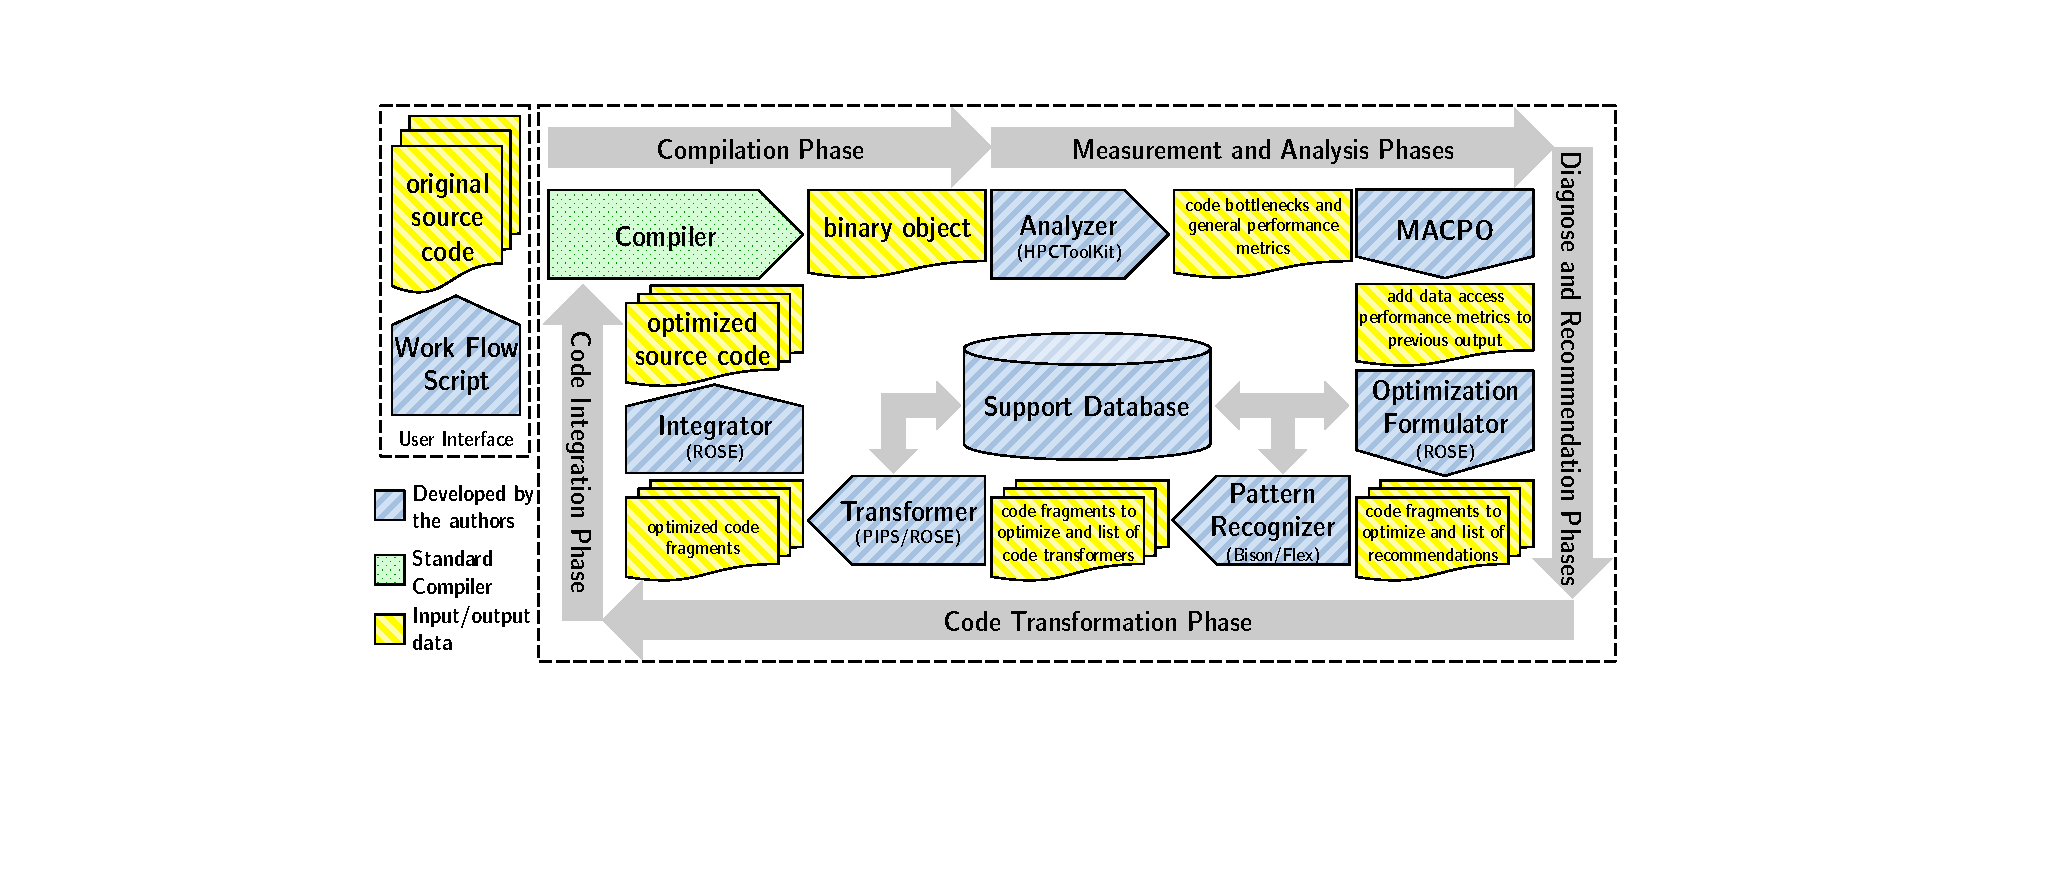
\includegraphics[width=12.8cm]{figures/pe_after}}
	\end{picture}
}

\frame{\frametitle{New Version: Work Flow Script}
	\begin{picture}(0,0)(0,0)
		\put(-28,-160){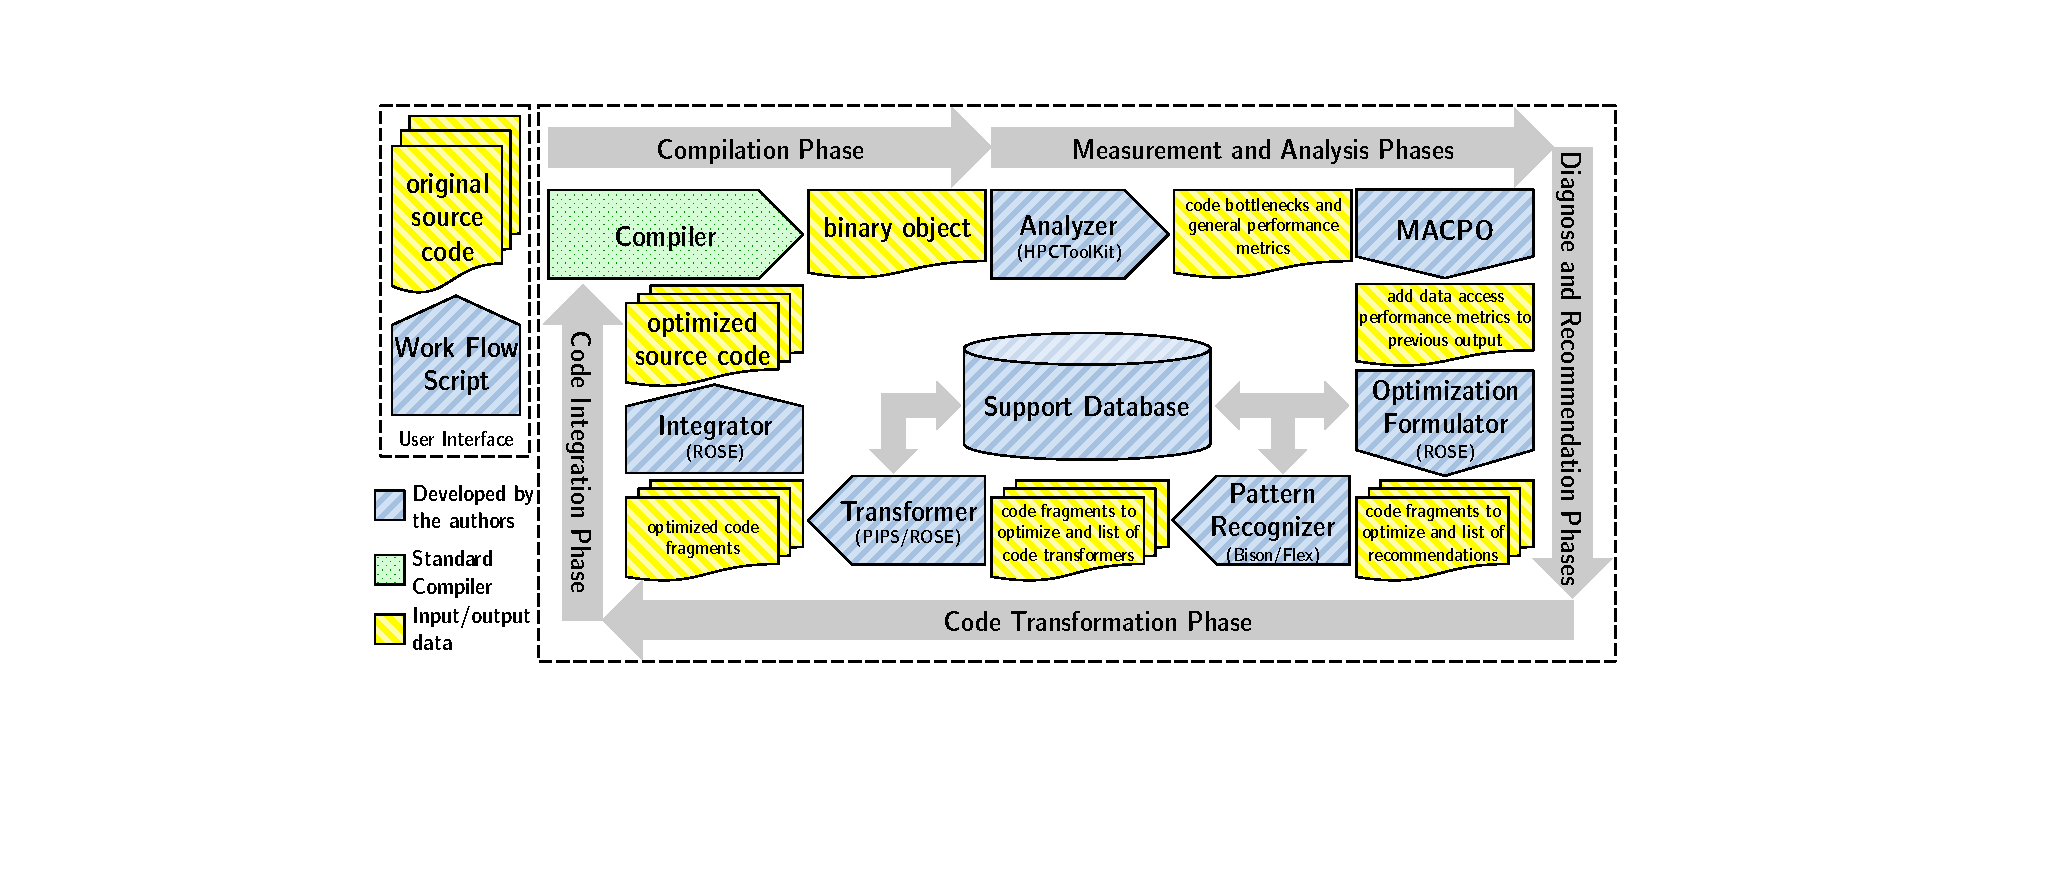
\includegraphics[width=12.8cm]{figures/pe_after}}
	\end{picture} %\pause
	\begin{columns}[c]
		\begin{column}{0.09\textwidth}
		\end{column}
		\begin{column}{0.43\textwidth}
			\vspace{1.5cm}
			\begin{block}{}
				\begin{itemize}
					\item This is a shell script \\[2mm] %\pause
					\item Accepts parameters \\[2mm] %\pause
					\item Invokes all tools (including the compiler) \\[2mm] %\pause
					\item Backward compatible \\[2mm]
				\end{itemize}
			\end{block}
		\end{column}
		\begin{column}{0.48\textwidth}
		\end{column}
	\end{columns}
}

\frame{\frametitle{New Version: Analyzer}
	\begin{picture}(0,0)(0,0)
		\put(-28,-160){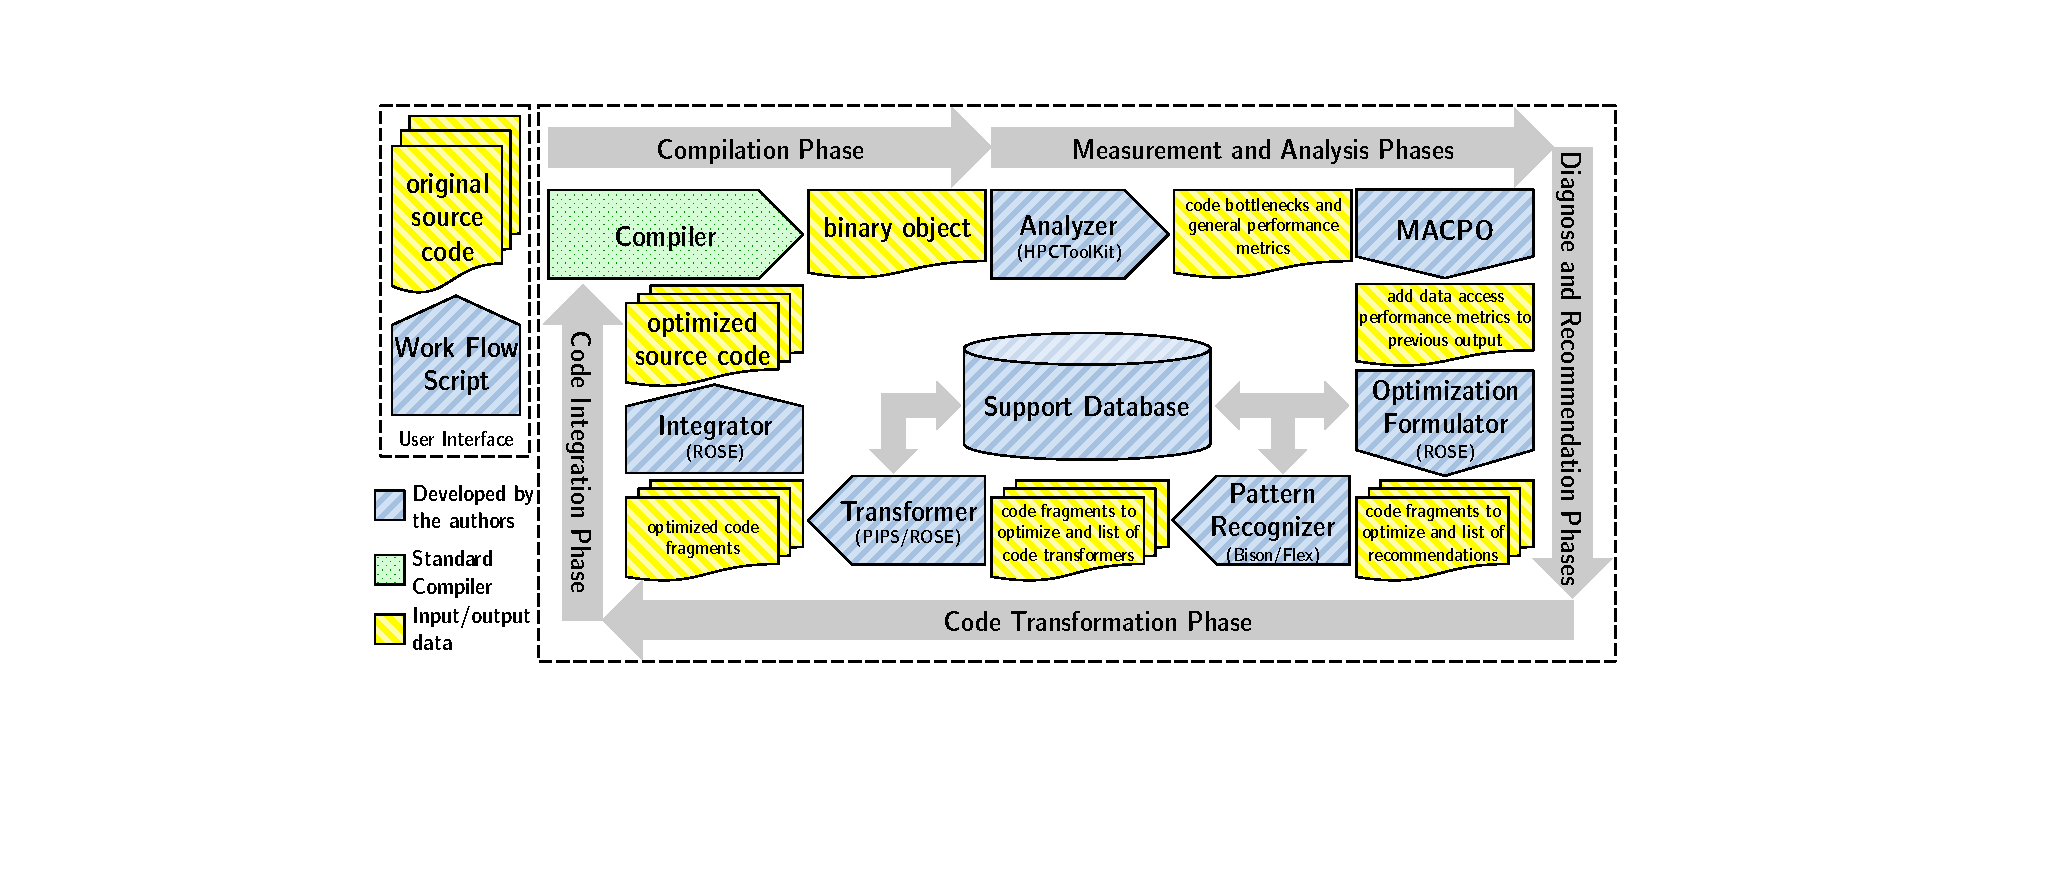
\includegraphics[width=12.8cm]{figures/pe_after}}
	\end{picture} %\pause
	\begin{columns}[c]
		\begin{column}{0.35\textwidth}
		\end{column}
		\begin{column}{0.46\textwidth}
			\vspace{1.5cm}
			\begin{block}{}
				\begin{itemize}
					\item This is the old PerfExpert, minus ``recommender'' \\[2mm] %\pause
					\item Based on HPCToolkit \\[2mm]
				\end{itemize}
			\end{block}
		\end{column}
		\begin{column}{0.19\textwidth}
		\end{column}
	\end{columns}
}

\frame{\frametitle{New Version: MACPO}
	\begin{picture}(0,0)(0,0)
		\put(-28,-160){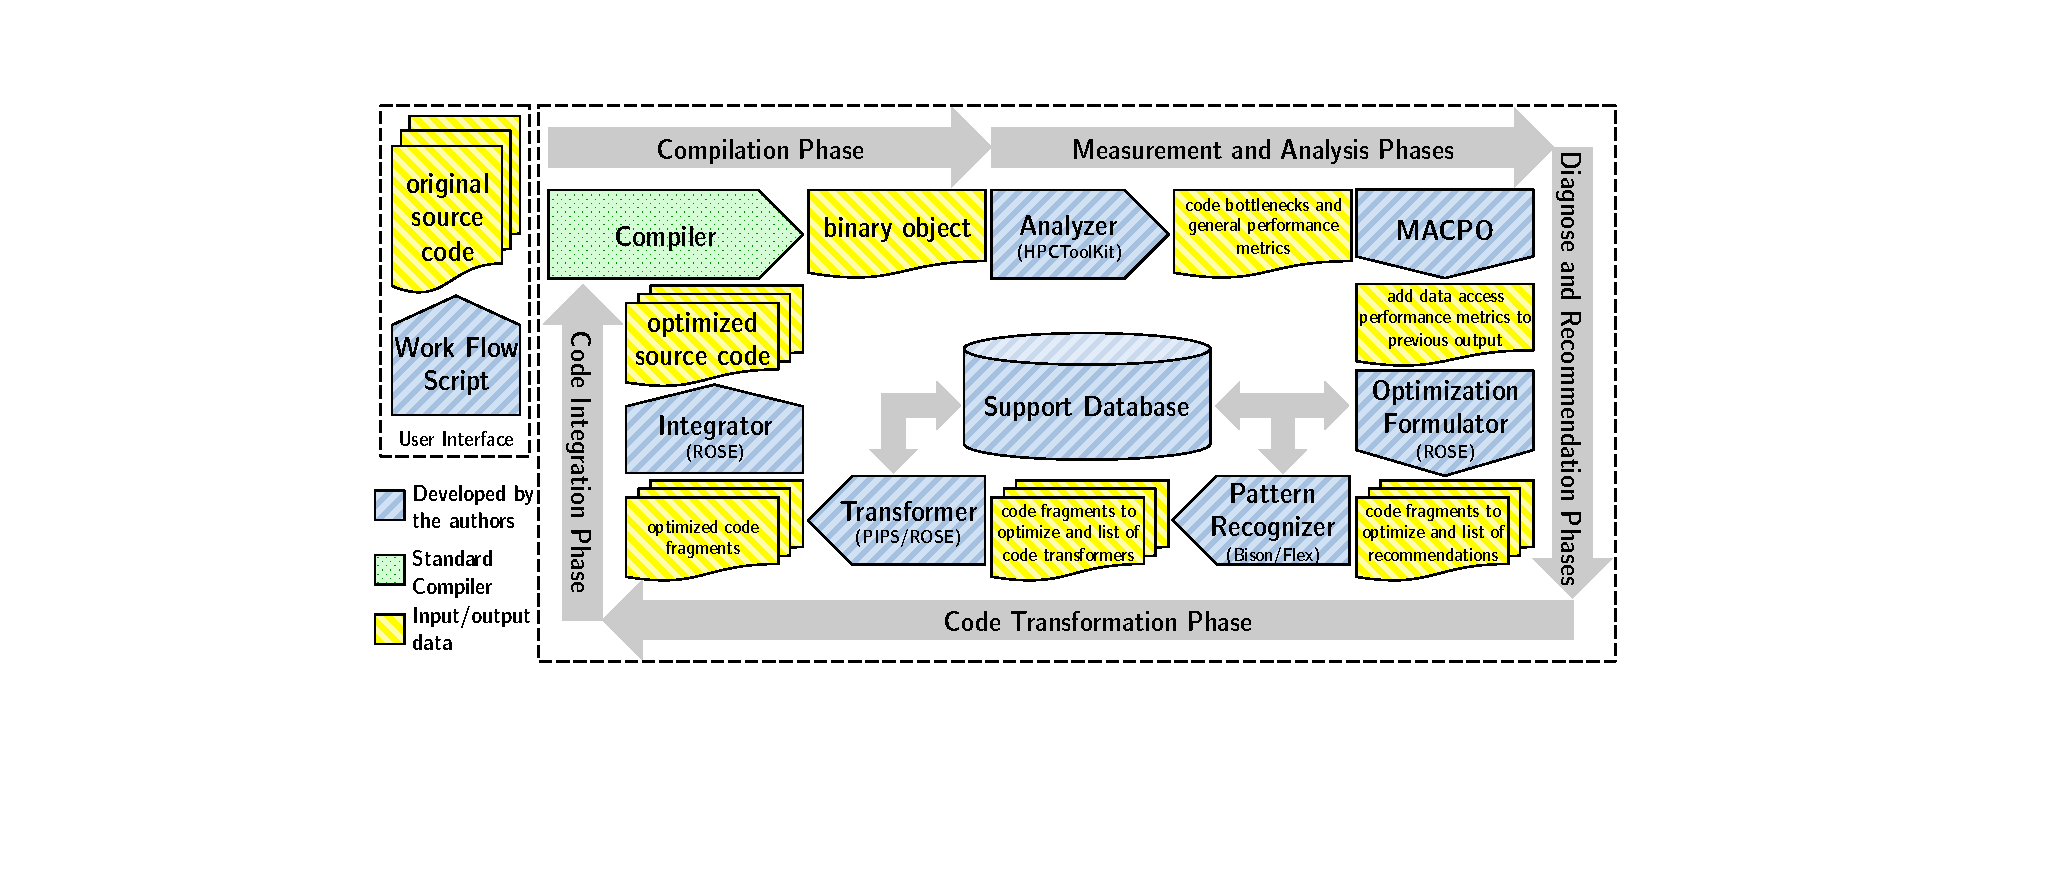
\includegraphics[width=12.8cm]{figures/pe_after}}
	\end{picture} %\pause
	\begin{columns}[c]
		\begin{column}{0.35\textwidth}
		\end{column}
		\begin{column}{0.46\textwidth}
			\vspace{1.5cm}
			\begin{block}{}
				\begin{itemize}
					\item Enhances the set of metrics with data access performance metrics \\[2mm] %\pause
					\item Based on ROSE \\[2mm]
				\end{itemize}
			\end{block}
		\end{column}
		\begin{column}{0.19\textwidth}
		\end{column}
	\end{columns}
}

\frame{\frametitle{New Version: Optimization Formulator}
	\begin{picture}(0,0)(0,0)
		\put(-28,-160){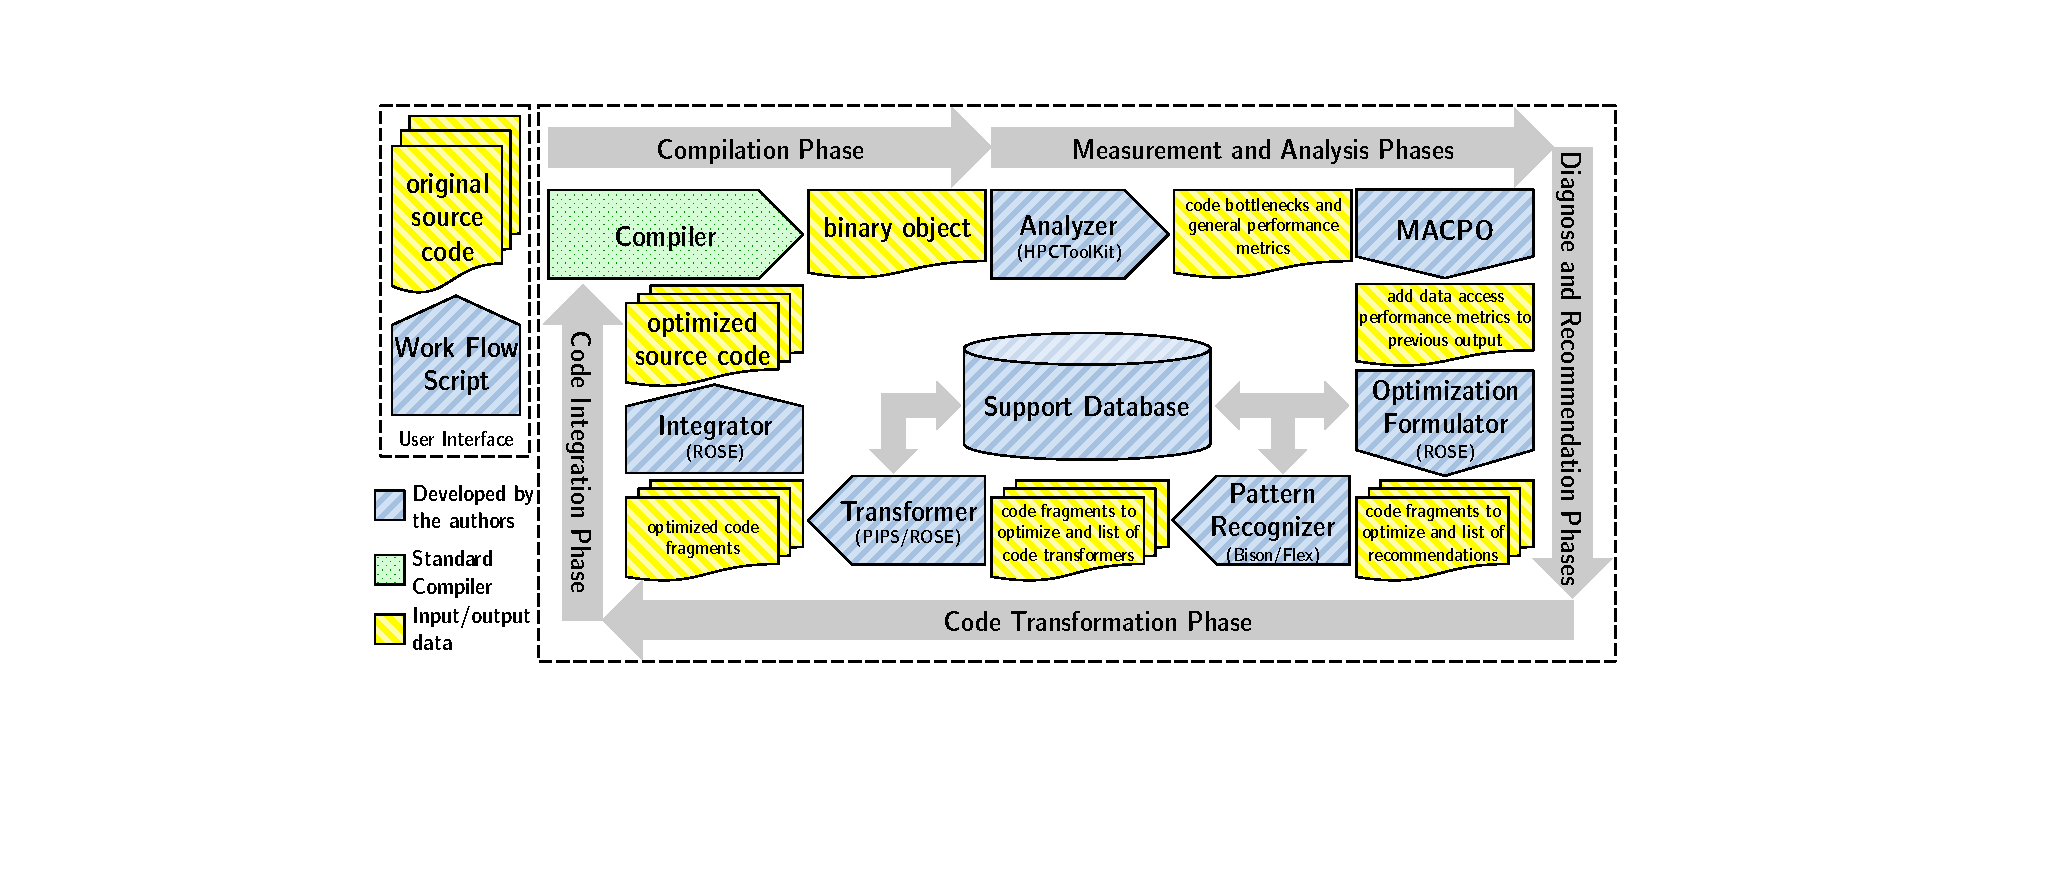
\includegraphics[width=12.8cm]{figures/pe_after}}
	\end{picture} %\pause
	\begin{columns}[c]
		\begin{column}{0.86\textwidth}
			\begin{block}{}
				\begin{itemize}
					\item Loads performance metrics on the Support Database \\[2mm] %\pause
					\item Runs all \textit{``recommendation selection functions''} \\[2mm] %\pause
					\item Concatenates and ranks the list of recommendations \\[2mm] %\pause
					\item Extracts code fragments identified as bottlenecks \\[2mm] %\pause
					\item Based on ROSE \\[2mm] %\pause
					\item \textbf{Extendable:} accepts user-defined performance metrics \\[2mm] %\pause
					\item \textbf{Extendable:} it is possible to write new \textit{``recommendation selection functions''} (SQL query) \\[2mm]
				\end{itemize}
			\end{block}
		\end{column}
		\begin{column}{0.19\textwidth}
		\end{column}
	\end{columns}
}

\frame{\frametitle{New Version: Support Database}
	\begin{picture}(0,0)(0,0)
		\put(-28,-160){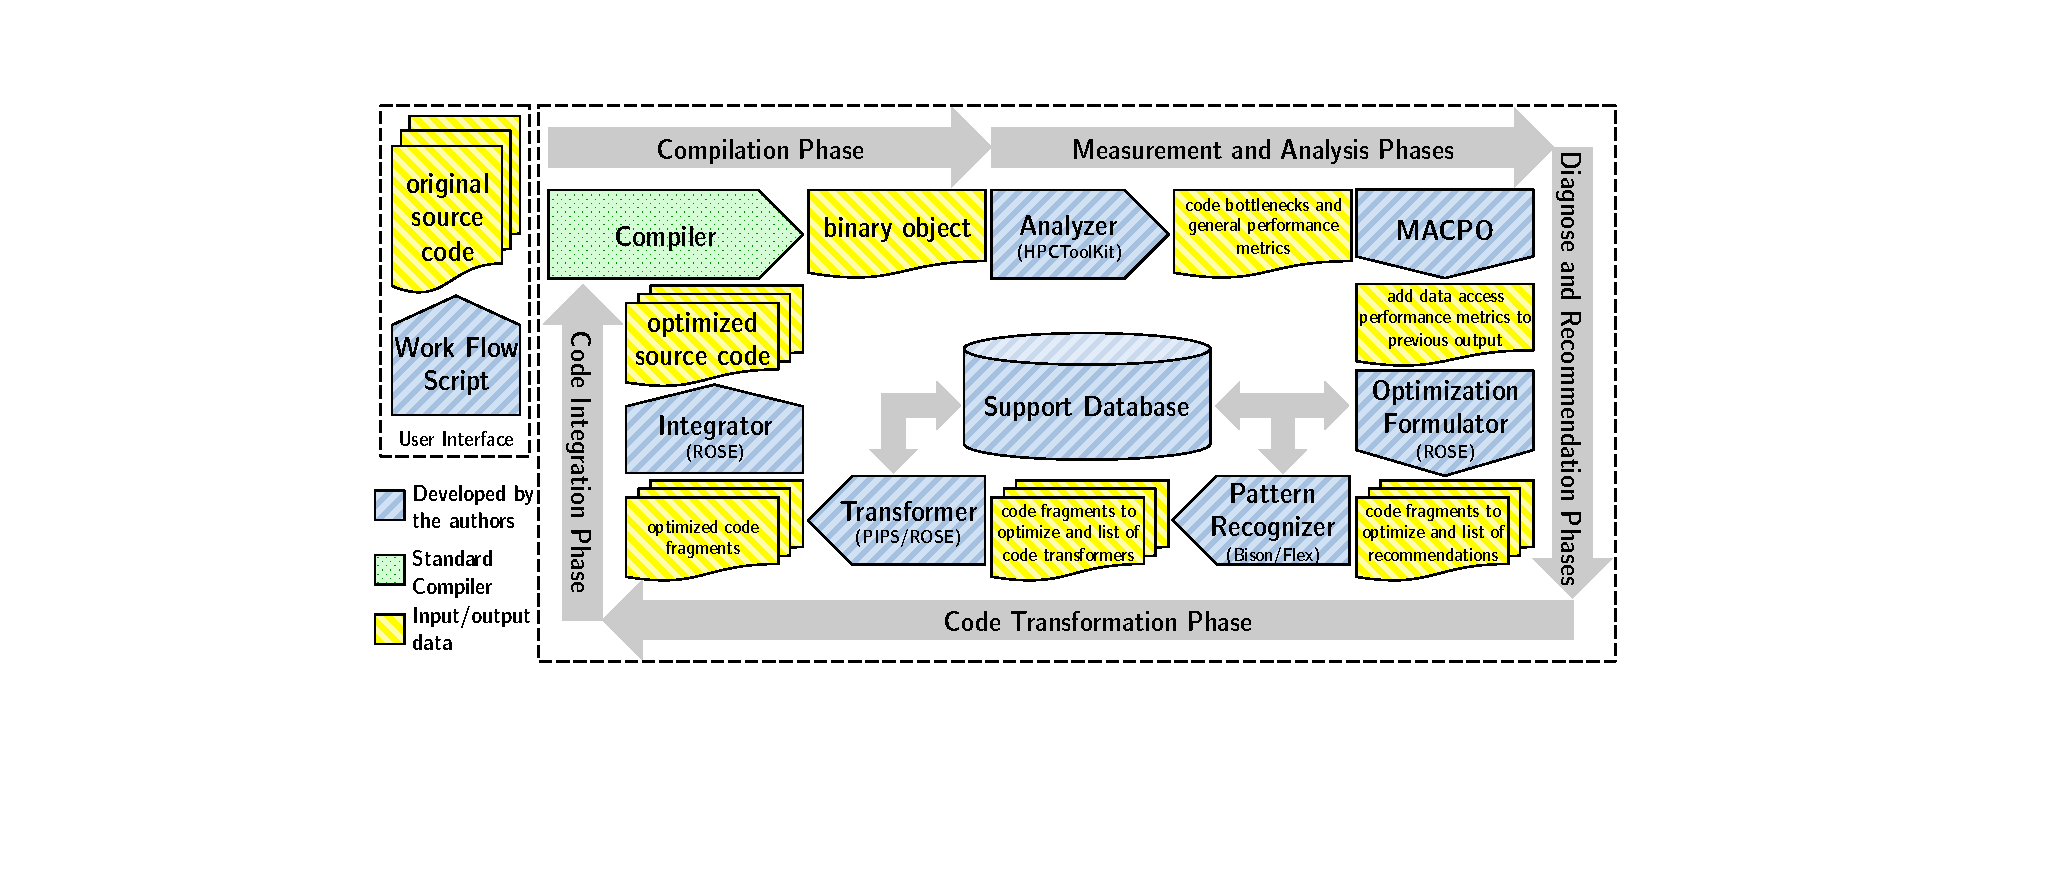
\includegraphics[width=12.8cm]{figures/pe_after}}
	\end{picture} %\pause
	\begin{columns}[c]
		\begin{column}{0.1\textwidth}
		\end{column}
		\begin{column}{0.96\textwidth}
			\vspace{-0.8cm}
			\begin{block}{}
				\begin{itemize}
					\item This is a SQLite database \\[2mm] %\pause
					\item Stores the list of \textit{``recommendation selection functions''}, \textit{``pattern recognizers''} and \textit{``code transformers''} \\[2mm] %\pause
					\item Engine to run the \textit{``recommendation selection functions''}
				\end{itemize}
			\end{block}
		\end{column}
	\end{columns}
}

\frame{\frametitle{New Version: Pattern Recognizer}
	\begin{picture}(0,0)(0,0)
		\put(-28,-160){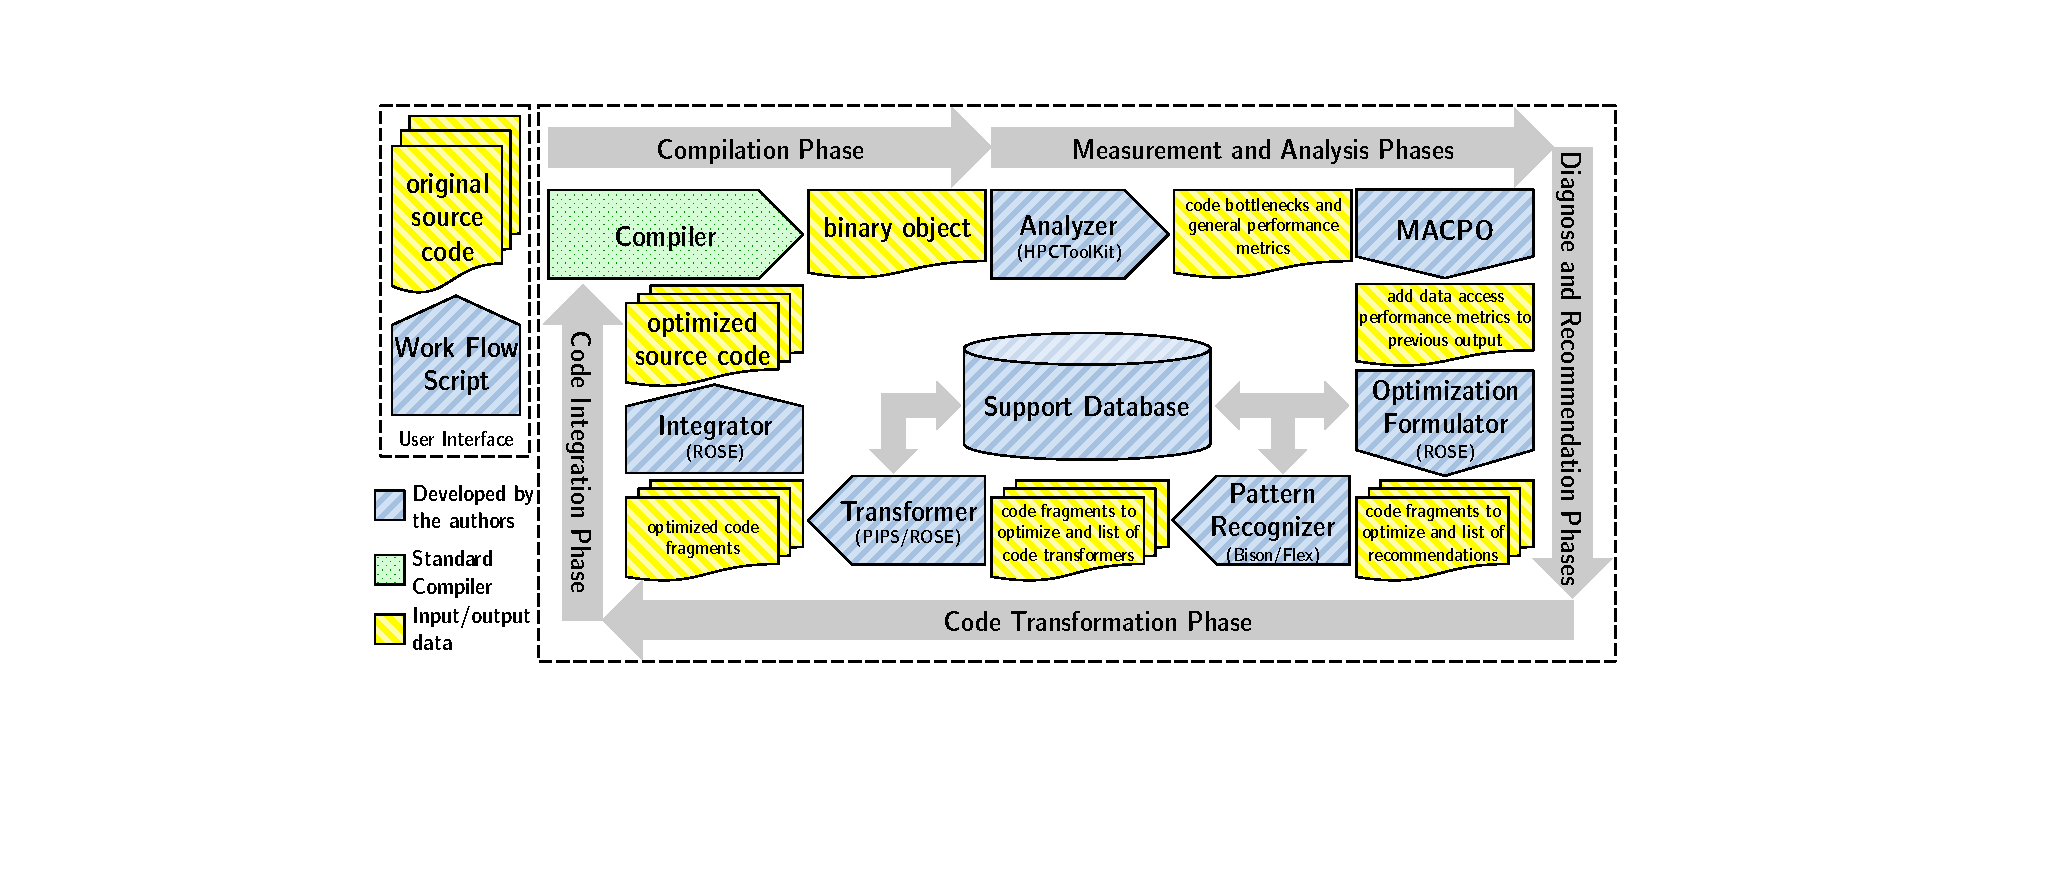
\includegraphics[width=12.8cm]{figures/pe_after}}
	\end{picture} %\pause
	\begin{columns}[c]
		\begin{column}{0.05\textwidth}
		\end{column}
		\begin{column}{1.05\textwidth}
			\vspace{-1.2cm}
			\begin{block}{}
				\begin{itemize}
					\item Acts as a ``filter'' trying to find (match) the right code transformer for a source code fragment (identified as bottleneck) \\[2mm] %\pause
					\item Language sensitive \\[2mm] %\pause
					\item Based on Bison and Flex \\[2mm] %\pause
					\item One recommendation may have multiple pattern recognizers \\[2mm] %\pause
					\item \textbf{Extendable:} it is possible to write new grammars to recognize/ match/filter code fragments (to work with new ``transformers'') \\[2mm]
				\end{itemize}
			\end{block}
		\end{column}
	\end{columns}
}

\frame{\frametitle{New Version: Transformer}
	\begin{picture}(0,0)(0,0)
		\put(-28,-160){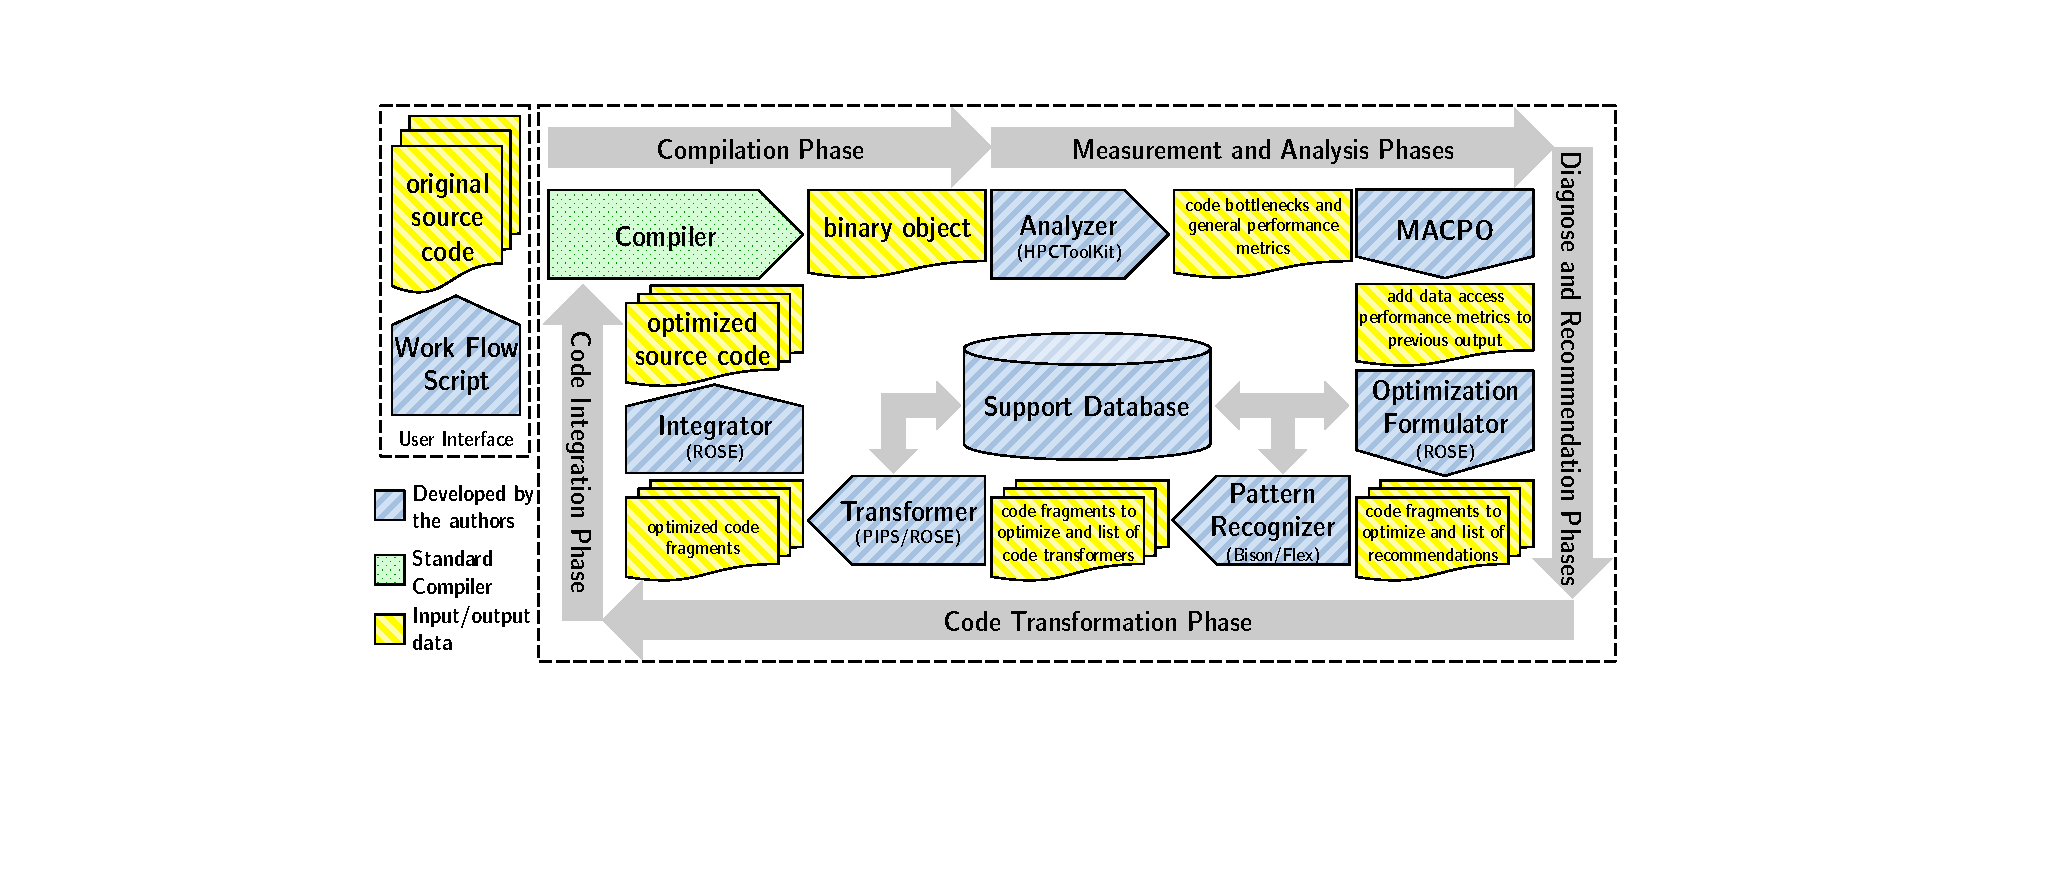
\includegraphics[width=12.8cm]{figures/pe_after}}
	\end{picture} %\pause
	\vspace{-1.1cm}
	\begin{block}{}
		\begin{itemize}
			\item Implements the recommendation by applying source code transformation \\[2mm] %\pause
			\item May or may not be language sensitive \\[2mm] %\pause
			\item Based on ROSE, PIPS or anything you want \\[2mm] %\pause
			\item One code pattern may lead to multiple code transformers \\[2mm] %\pause
			\item \textbf{Extendable:} it is possible to write code transformers using any language you want \\[2mm]
		\end{itemize}
	\end{block}
}

\frame{\frametitle{New Version: Integrator}
	\begin{picture}(0,0)(0,0)
		\put(-28,-160){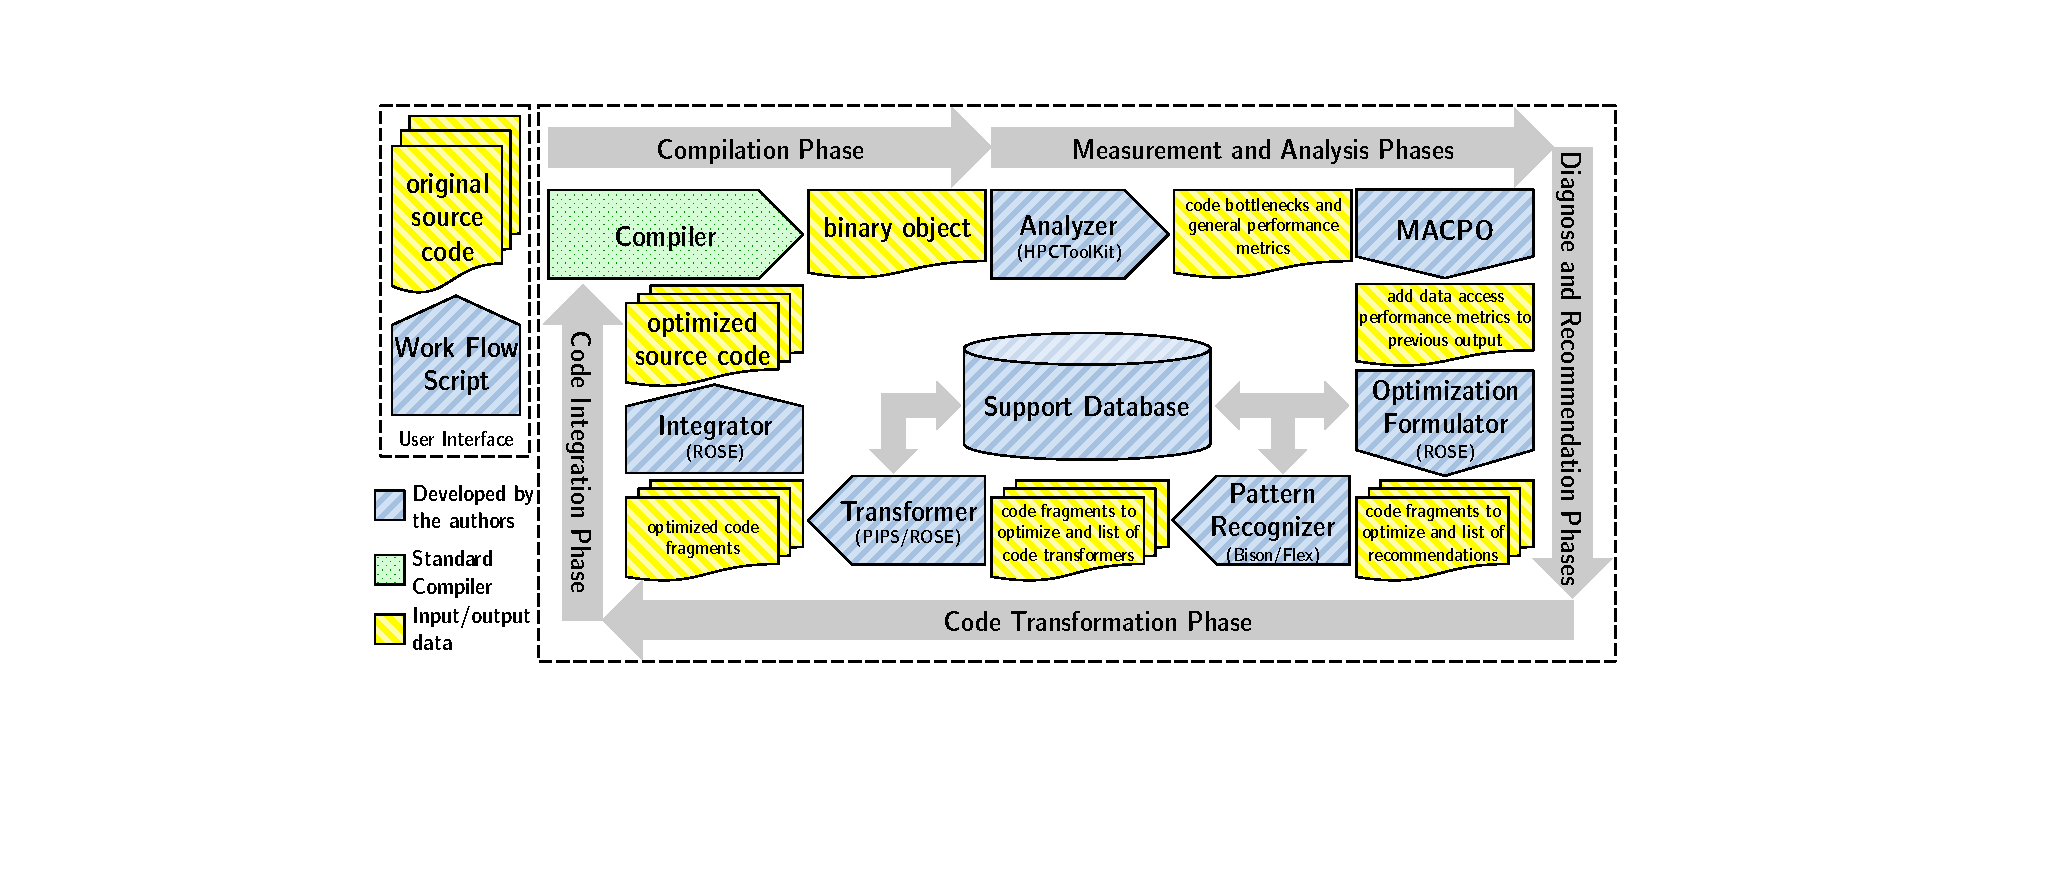
\includegraphics[width=12.8cm]{figures/pe_after}}
	\end{picture} %\pause
	\begin{columns}[c]
		\begin{column}{0.35\textwidth}
		\end{column}
		\begin{column}{0.46\textwidth}
			\vspace{1.5cm}
			\begin{block}{}
				\begin{itemize}
					\item Generates a new source code by integrating to the transformed code fragments \\[2mm] %\pause
					\item Based on ROSE \\[2mm]
				\end{itemize}
			\end{block}
		\end{column}
		\begin{column}{0.19\textwidth}
		\end{column}
	\end{columns}
}

%------------------------------------------------------------
\section{Understanding and Extending PerfExpert}
\subsection{Understanding and Extending PerfExpert}

\frame{\frametitle{Understanding PerfExpert Analysis}
	\begin{block}{On the The Analysis Report...} %\pause
		\begin{itemize}
			\item The more ``expensive'' comes first \\[2mm] %\pause
			\item Tells user where the slow code sections are as well as why they perform poorly \\[2mm] %\pause
			\item Every function or loop which takes more than 1\% of the execution time is analyzed (default value) \\[2mm] %\pause
			\item Yes, we rely on performance metrics (but not only and not the raw ones) \\[2mm] %\pause
			\item No, we do not rely on hardware specs \\[2mm] %\pause
			\item If you are not using properly the node PerfExpert may conclude everything is fine (use a representative workload) \\[2mm] %\pause
		\end{itemize}
	\end{block}
}

\frame{\frametitle{Performance Report}
	\begin{block}{}
\texttt{\tiny Loop in function compute() at mm.c:8 (99.8\% of the total runtime)\\
===============================================================================\\
ratio to total instrns \ \ \ \ \ \ \%  0.........25...........50.........75........100\\
\ \ \ - floating point \ \ \ \ \ : \ 100 ***********************************************\\
\ \ \ - data accesses \ \ \ \ \ \ : \ \ 25 ************\\
* GFLOPS (\% max) \ \ \ \ \ \ \ \ : \ \ 12 ******\\
\ \ \ - packed \ \ \ \ \ \ \ \ \ \ \ \ \ : \ \ \ 0 *\\
\ \ \ - scalar \ \ \ \ \ \ \ \ \ \ \ \ \ : \ \ 12 ******\\
-------------------------------------------------------------------------------\\
performance assessment \ \ \ \ \ LCPI good......okay......fair......poor......bad....\\
* overall \ \ \ \ \ \ \ \ \ \ \ \ \ \ \ : \ 3.0 >>>>>>>>>>>>>>>>>>>>>>>>>>>>>>>>>>>>>>>>>>>>>>+\\
upper bound estimates\\
* data accesses \ \ \ \ \ \ \ \ \ : \ 9.6 >>>>>>>>>>>>>>>>>>>>>>>>>>>>>>>>>>>>>>>>>>>>>>+\\
\ \ \ - L1d hits \ \ \ \ \ \ \ \ \ \ \ : \ 0.9 >>>>>>>>>>>>>>>>>\\
\ \ \ - L2d hits \ \ \ \ \ \ \ \ \ \ \ : \ 1.8 >>>>>>>>>>>>>>>>>>>>>>>>>>>>>>>>>>>>>\\
\ \ \ - L2d misses \ \ \ \ \ \ \ \ \ : \ 6.9 >>>>>>>>>>>>>>>>>>>>>>>>>>>>>>>>>>>>>>>>>>>>>>+\\
* instruction accesses \ \ : \ 0.1 >\\
\ \ \ - L1i hits \ \ \ \ \ \ \ \ \ \ \ : \ 0.0 >\\
\ \ \ - L2i hits \ \ \ \ \ \ \ \ \ \ \ : \ 0.0 >\\
\ \ \ - L2i misses \ \ \ \ \ \ \ \ \ : \ 0.1 >\\
* data TLB \ \ \ \ \ \ \ \ \ \ \ \ \ \ : \ \ 4.6 >>>>>>>>>>>>>>>>>>>>>>>>>>>>>>>>>>>>>>>>>>>>>>+\\
* instruction TLB \ \ \ \ \ \ \ : \ \ 0.0 >\\
* branch instructions \ \ \ : \ 0.1 >>\\
\ \ \ - correctly predicted : \ 0.1 >>\\
\ \ \ - mispredicted \ \ \ \ \ \ \ : \ 0.0 >\\
* floating-point instr \ \ : \ 5.1 >>>>>>>>>>>>>>>>>>>>>>>>>>>>>>>>>>>>>>>>>>>>>>+\\
\ \ \ - fast FP instr \ \ \ \ \ \ : \ 5.1 >>>>>>>>>>>>>>>>>>>>>>>>>>>>>>>>>>>>>>>>>>>>>>+\\
\ \ \ - slow FP instr \ \ \ \ \ \ : \ 0.0 >\\
}
   \end{block}
}

\frame{\frametitle{Metrics used by PerfExpert} %\pause
	\vspace{-5mm}
	\begin{block}{Architecture Characteristics} %\pause
		\begin{itemize}
			\item Memory access latency: L1, L2, L3 and main memory (based on micro-benchmarks) \\[0mm] %\pause
			\item Memory topology and size (based on hwlock) \\[0mm] %\pause
			\item Branch latency and missed branch latency (based on micro-benchmarks) \\[0mm] %\pause
			\item Float-point operation latency (based on micro-benchmarks) \\[0mm] %\pause
			\item Micro-architecture \textcolor{red}{(in progress)} \\[0mm]
		\end{itemize}
	\end{block}
	\vspace{-2mm}
	\begin{block}{Source Code} %\pause
		\begin{itemize}
			\item Language (C, C++, Fortran) \\[0mm] %\pause
			\item File name and line number \\[0mm] %\pause
			\item Type (loop or function) \\[0mm] %\pause
			\item Function name and ``deepness'' \\[0mm] %\pause
			\item Representativeness (percentage of execution time) \\[0mm]
		\end{itemize}
	\end{block}
}

\frame{\frametitle{Metrics used by PerfExpert} %\pause
	\begin{block}{Execution Performance} %\pause
		\begin{itemize}
			\item Raw data (PAPI) \\[2mm] %\pause
			\item LCPI: local cycles per instruction (PerfExpert Analyzer) \\[2mm]
		\end{itemize}
	\end{block}
	\begin{block}{Data Access Performance (from MACPO)} %\pause
		\begin{itemize}
			\item Access strides and the frequency of occurrence (*) \\[2mm] %\pause
			\item Presence or absence of cache thrashing and the frequency (*) \\[2mm] %\pause
			\item Estimated cost (cycles) per access (*) \\[2mm] %\pause
			\item NUMA misses (*) \\[2mm] %\pause
			\item Reuse factors for data caches (*) \\[2mm] %\pause
			\item Stream count \\[2mm]
		\end{itemize}
	\end{block}
	(*) \textit{per variable}
}

\subsection{Extending PerfExpert}

\frame{\frametitle{Extending PerfExpert} %\pause
	\vspace{-4mm}
	\begin{block}{Adding Performance Metrics} %\pause
		\begin{itemize}
			\item Dynamically loaded into the support database \\[2mm] %\pause
			\item We treat everything (most of them, actually) as metrics \\[2mm] %\pause
		\end{itemize}
	\end{block}
	\begin{exampleblock}{Some Example Metrics} %\pause
		\texttt{\small code.section\_info=Loop in function compute() at mm.c:8\\
code.filename=mm.c\\
code.line\_number=8\\
code.type=loop\\
code.function\_name=compute\\
code.representativeness=99.8\\
perfexpert.ratio.data\_accesses=0.25\\
perfexpert.instruction\_accesses.L2i\_hits=0.002\\
perfexpert.branch\_instructions.mispredicted=0.0\\
perfexpert.floating-point\_instr.fast\_FP\_instr=5.073\\
perfexpert.data\_accesses.L2d\_hits=1.846\\...\\}
	\end{exampleblock}
}

\frame{\frametitle{Extending PerfExpert} %\pause
	\begin{block}{Recommendation Selection Functions} %\pause
		\begin{itemize}
			\item Is is just a SQL query \\[2mm] %\pause
			\item You can use as many functions as you want \\[2mm] %\pause
			\item We already have some strategies on how to rank recommendations \\[2mm] %\pause
			\item A recommendation may lead to several pattern recognizers \\[2mm] %\pause
		\end{itemize}
	\end{block}
	\begin{exampleblock}{A Simple Recommendation Selection Function Example} %\pause
		\centering\texttt{SELECT recommendation FROM t\_rec WHERE \\
metric.A > `this' AND metric.B <= `that' \\
ORDER BY score DESC;
}
	\end{exampleblock}
}

\frame{\frametitle{Extending PerfExpert} %\pause
	\begin{block}{Pattern Recognizers} %\pause
		\begin{itemize}
			\item Any program which returns \texttt{0} or  \texttt{1} \\[2mm] %\pause
			\item Language sensitive \\[2mm] %\pause
			\item A pattern recognizer may lead to several code transformers \\[2mm] %\pause
		\end{itemize}
	\end{block}
	\begin{exampleblock}{A Simple Grammar (Byson/Flex)} %\pause
		\texttt{\tiny nested\_iteration\_statement\\
 : WHILE '(' exp ')' WHILE '(' exp ')' stmnt\\
 | WHILE '(' exp ')' '{' WHILE '(' exp ')' stmnt '}'\\
 | DO DO stmnt WHILE '(' exp ')' ';' stmnt WHILE '(' exp ')' ';'\\
 | DO '{' DO stmnt WHILE '(' exp ')' ';' '}' WHILE '(' exp ')' ';'\\
 | FOR '(' exp\_stmnt exp\_stmnt ')' FOR '(' exp\_stmnt exp\_stmnt ')' stmnt\\
 | FOR '(' exp\_stmnt exp\_stmnt ')' '{' FOR '(' exp\_stmnt exp\_stmnt ')' stmnt '}'\\
 | FOR '(' exp\_stmnt exp\_stmnt exp ')' FOR '(' exp\_stmnt exp\_stmnt exp ')' stmnt\\
 | FOR '(' exp\_stmnt exp\_stmnt exp ')' '{' FOR '(' exp\_stmnt exp\_stmnt exp ')' stmnt '}' ;\\
}
	\end{exampleblock}
}

\frame{\frametitle{Extending PerfExpert} %\pause
	\begin{block}{Code Transformers} %\pause
		\begin{itemize}
			\item Any program which returns \texttt{0} or  \texttt{1} \\[2mm] %\pause
			\item May be language sensitive \\[2mm] %\pause
		\end{itemize}
	\end{block}
	\begin{exampleblock}{A Simple TPIPS script} %\pause
		\texttt{\small create c\_loop2 ../source/mm.c\\
activate INTERPROCEDURAL\_SUMMARY\_PRECONDITION\\
activate TRANSFORMERS\_INTER\_FULL\\
activate PRECONDITIONS\_INTER\_FULL\\
setproperty SEMANTICS\_FIX\_POINT\_OPERATOR ``derivative''\\
module compute\\
apply LOOP\_INTERCHANGE\\
loop\_8\\
apply UNSPLIT[\%PROGRAM]\\
close\\
quit\\
}
	\end{exampleblock}
}

%------------------------------------------------------------
\section{Conclusions}
\subsection{Conclusions}
\frame{\frametitle{Conclusions} %\pause
	\begin{block}{Why is this performance optimization ``architecture'' strong?} %\pause
		\begin{itemize}\small
			\item Each piece of the tool chain can be updated/upgraded individually \\[0mm] %\pause
			\item \textbf{It is extendable}: metrics, performance measurement and analysis phases, recommendations, transformations and strategies to select recommendations \\[0mm] %\pause
			\item Multi-language, \textbf{multi-architecture}, open-source and built on top of well-established tools (HPCToolkit, ROSE, PIPS, etc.) \\[0mm] %\pause
			\item Easy to use and lightweight!
		\end{itemize}
	\end{block}
	\begin{block}{}
		\begin{itemize}\small
			\item This is the first end-to-end open-source performance optimization tool (as far as we know)\\[0mm] %\pause
			\item It will become more and more powerful as new recommendations, transformations and features are added \\[0mm] %\pause
			\item There is no ``big code'' (to increase in complexity until it become unusable or too hard to maintain) \\[0mm]
		\end{itemize}
	\end{block}
}

\frame{\frametitle{Next Steps} %\pause
	\vspace{-3mm}
	\begin{block}{Major Goals} %\pause
		\begin{itemize}\small
			\item Improve analysis based on the data access \textcolor{red}{(in progress)} \\[0mm] %\pause
			\item Increase the number of recommendations and possible code transformations \textcolor{red}{(continuously)} \\[0mm] %\pause
			\item New algorithms for recommendations selection \textcolor{red}{(in progress)} \\[0mm] %\pause
			\item Add support to MIC architecture \textcolor{red}{(in progress)} \\[0mm] %\pause
			\item Add support to MPI-related recommendations (medium term) \\[0mm] %\pause
			\item Add support to MPI-related code transformations (long term) \\[0mm] %\pause
		\end{itemize}
	\end{block}
	\begin{block}{Minor Goals} %\pause
		\begin{itemize}\small
			\item Support ``Makefile''-based source code/compilation tree \textcolor{red}{(done!)} \\[0mm] %\pause
			\item Make the required packages installation process easier \textcolor{red}{(done!)} \\[0mm] %\pause
			\item Add a test suite based on established benchmark codes \textcolor{red}{(in progress)} \\[0mm] %\pause
			\item Easy-to-use interface to manipulate the support database (medium term) \\[0mm]
		\end{itemize}
	\end{block}
}

\frame[plain]{
	\vspace{1cm}
	\begin{center}
		\textbf{\Huge{Thank You\\ \ \\ fialho@utexas.edu}} \\
		\vspace{1cm}
		\textbf{\LARGE{http://www.tacc.utexas.edu/perfexpert}}
	\end{center}
%	\vspace{1cm}
	\pgfuseimage{logo_TACC} \ \ \pgfuseimage{logo_UT}
}

%------------------------------------------------------------
\end{document}